\subsection{$\nu_{\mu}$ Events}
\label{sec:NuMuSideband}

This sideband is obtained by applying the full muon neutrino event selection described in Section~\ref{sec:EventSelections}. This sideband is used to constrain the prediction in the signal region. Predictions are compared to data from the different epochs in Figure~\ref{fig:NuMuSideband}, for the reconstructed muon energy, muon candidate direction, and reconstructed neutrino energy, showing agreement within uncertainties in all three variables, and good stability across the runs.

\begin{figure}[H]
    \centering
    \begin{subfigure}{0.33\linewidth}
        \captionsetup{width=0.7\linewidth}
        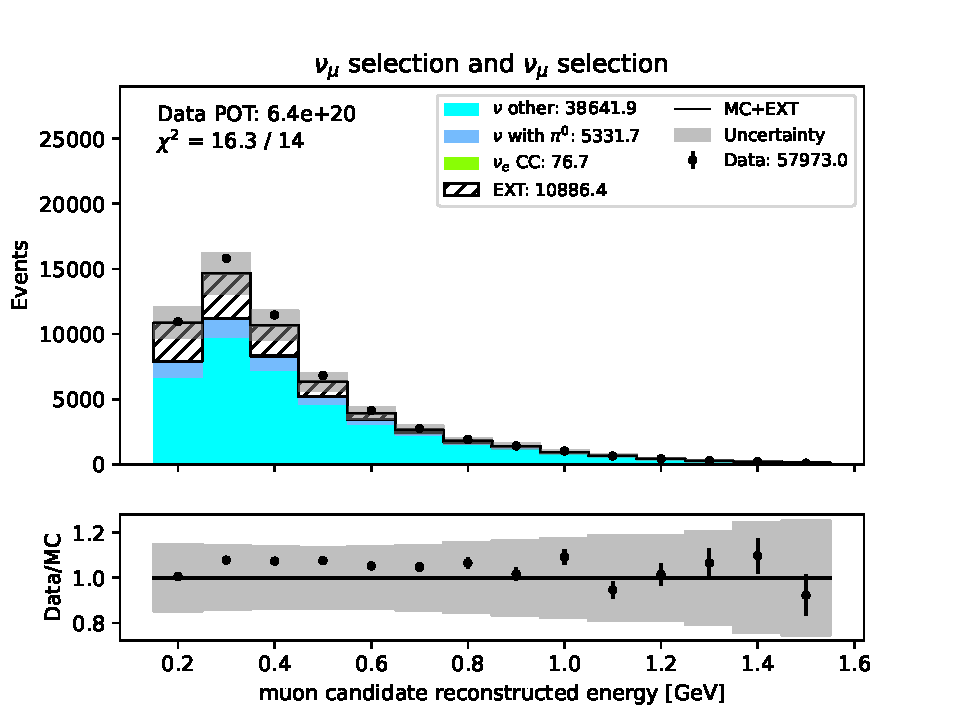
\includegraphics[width=\linewidth]{technote/Sidebands/Figures/NuMuSideband/muon_sideband_muon_energy_run123_NUMU_NUMU.pdf}
        \caption{Muon reconstructed energy, runs 1-3.}
    \end{subfigure}%
    \begin{subfigure}{0.33\linewidth}
        \captionsetup{width=0.6\linewidth}
        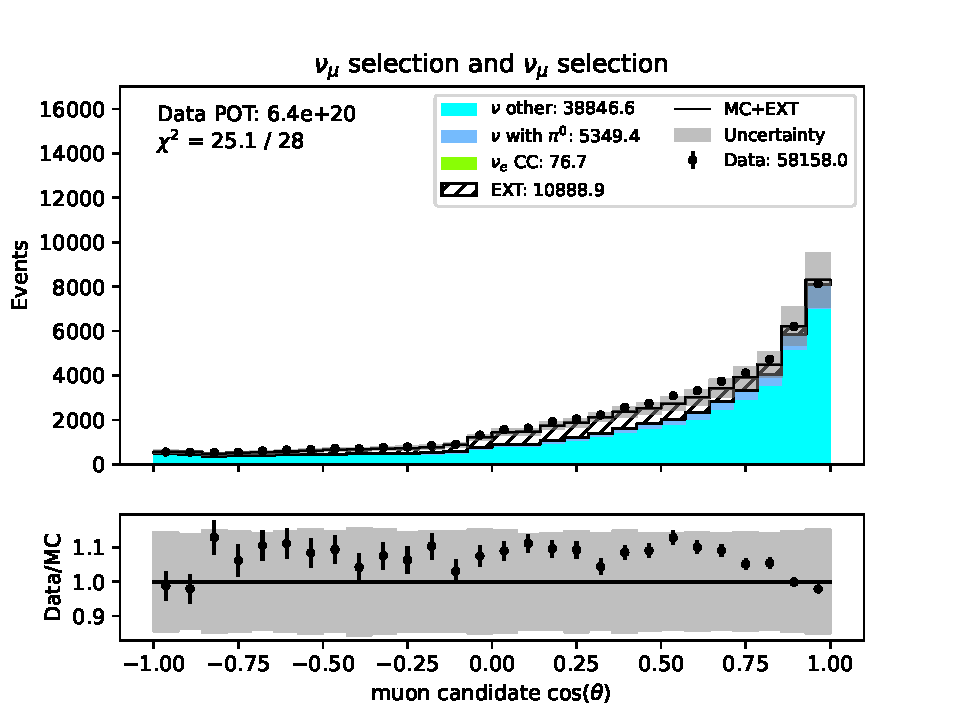
\includegraphics[width=\linewidth]{technote/Sidebands/Figures/NuMuSideband/muon_sideband_muon_theta_run123_NUMU_NUMU.pdf}
        \caption{Muon candidate direction, runs 1-3.}
    \end{subfigure}%
    \begin{subfigure}{0.33\linewidth}
        \captionsetup{width=0.7\linewidth}
        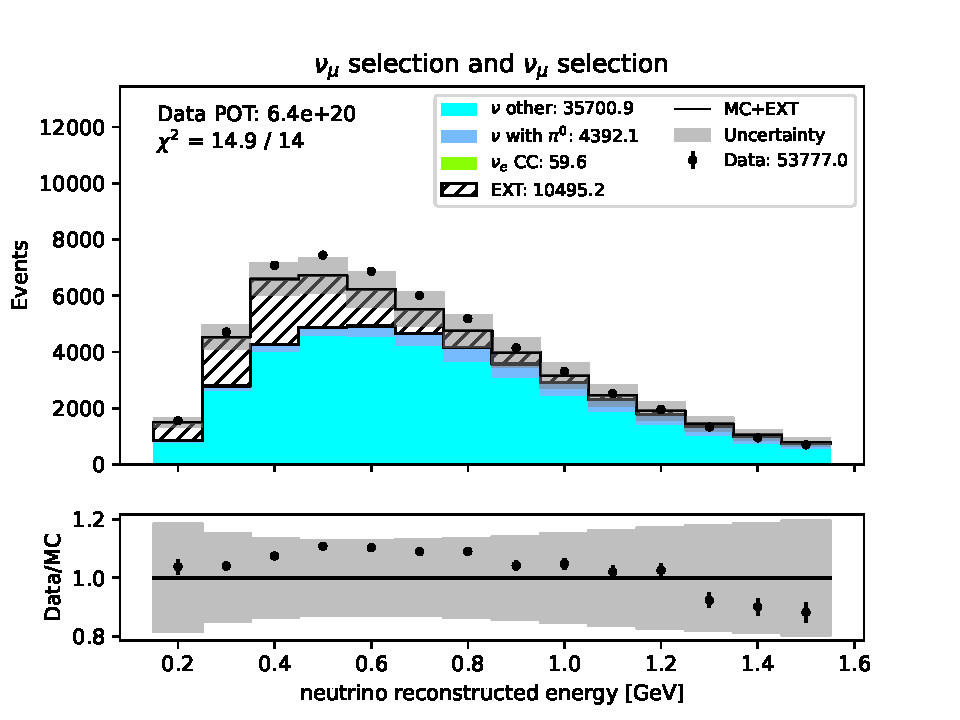
\includegraphics[width=\linewidth]{technote/Sidebands/Figures/NuMuSideband/muon_sideband_neutrino_energy_run123_NUMU_NUMU.pdf}
        \caption{Reconstructed neutrino energy, runs 1-3.}
    \end{subfigure}
    \begin{subfigure}{0.33\linewidth}
        \captionsetup{width=0.7\linewidth}
        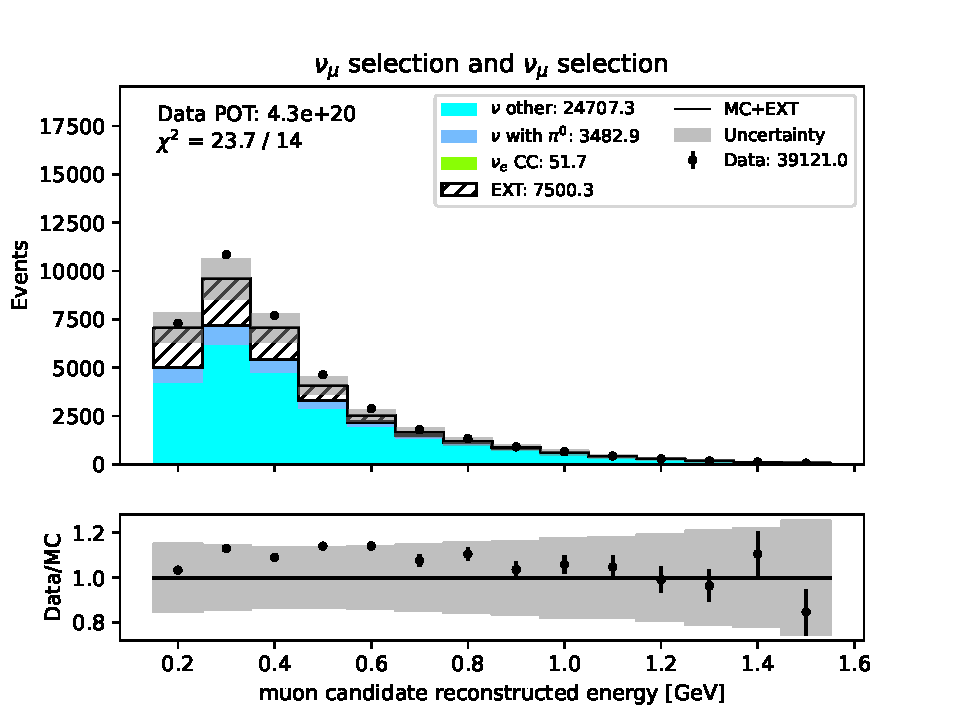
\includegraphics[width=\linewidth]{technote/Sidebands/Figures/NuMuSideband/muon_sideband_muon_energy_run4b4c4d5_NUMU_NUMU.pdf}
        \caption{Muon reconstructed energy, runs 4-5.}
    \end{subfigure}%
    \begin{subfigure}{0.33\linewidth}
        \captionsetup{width=0.6\linewidth}
        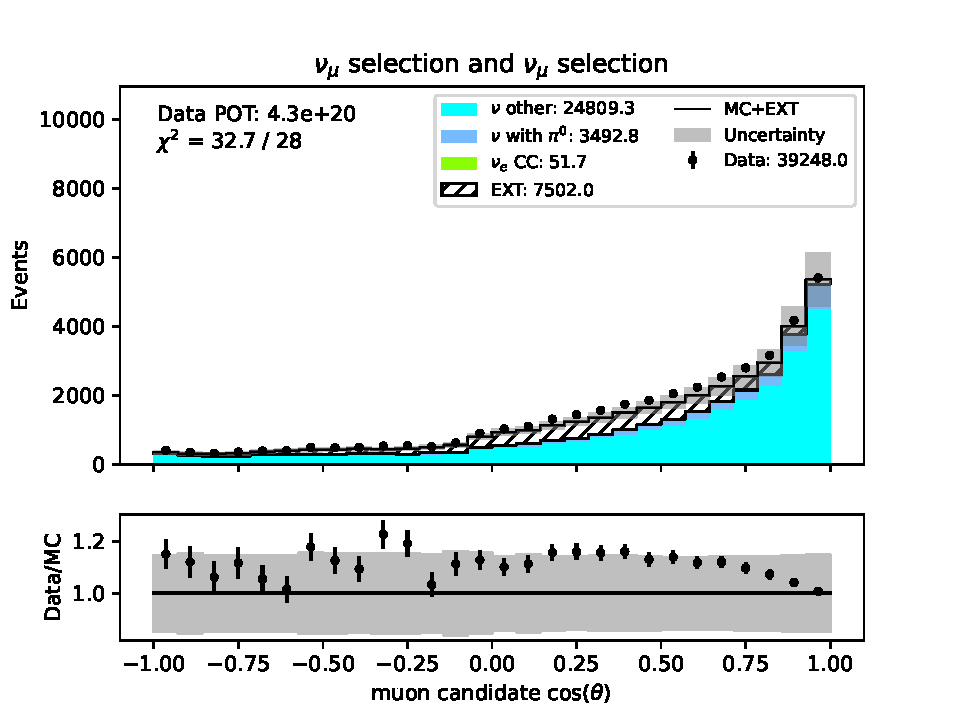
\includegraphics[width=\linewidth]{technote/Sidebands/Figures/NuMuSideband/muon_sideband_muon_theta_run4b4c4d5_NUMU_NUMU.pdf}
        \caption{Muon candidate direction, runs 4-5.}
    \end{subfigure}%
    \begin{subfigure}{0.33\linewidth}
        \captionsetup{width=0.7\linewidth}
        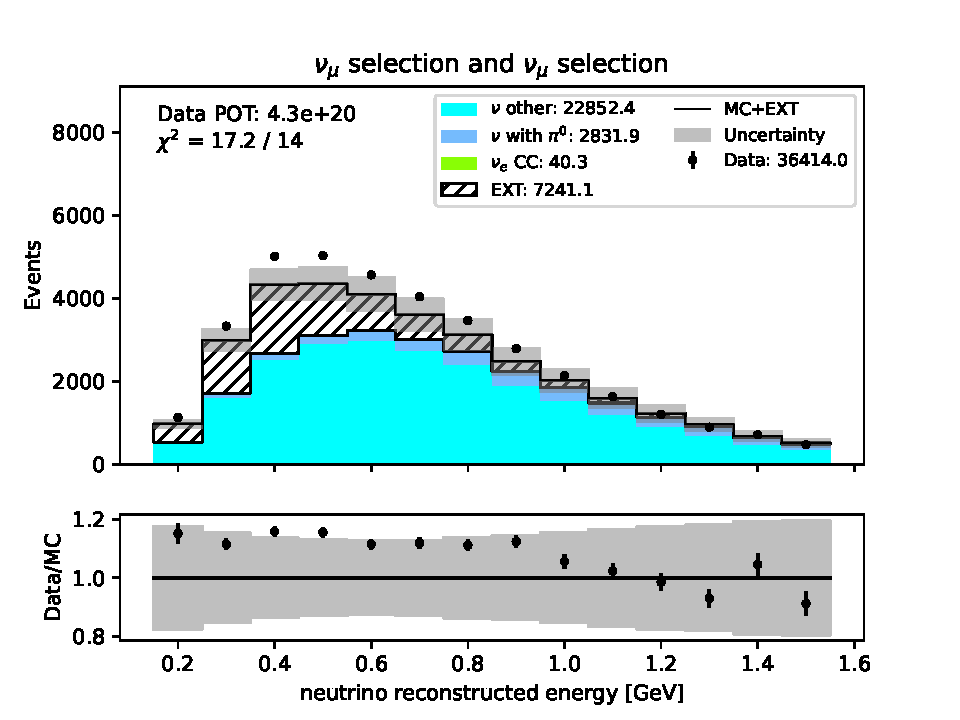
\includegraphics[width=\linewidth]{technote/Sidebands/Figures/NuMuSideband/muon_sideband_neutrino_energy_run4b4c4d5_NUMU_NUMU.pdf}
        \caption{Reconstructed neutrino energy, runs 4-5.}
    \end{subfigure}    
    \begin{subfigure}{0.33\linewidth}
        \captionsetup{width=0.7\linewidth}
        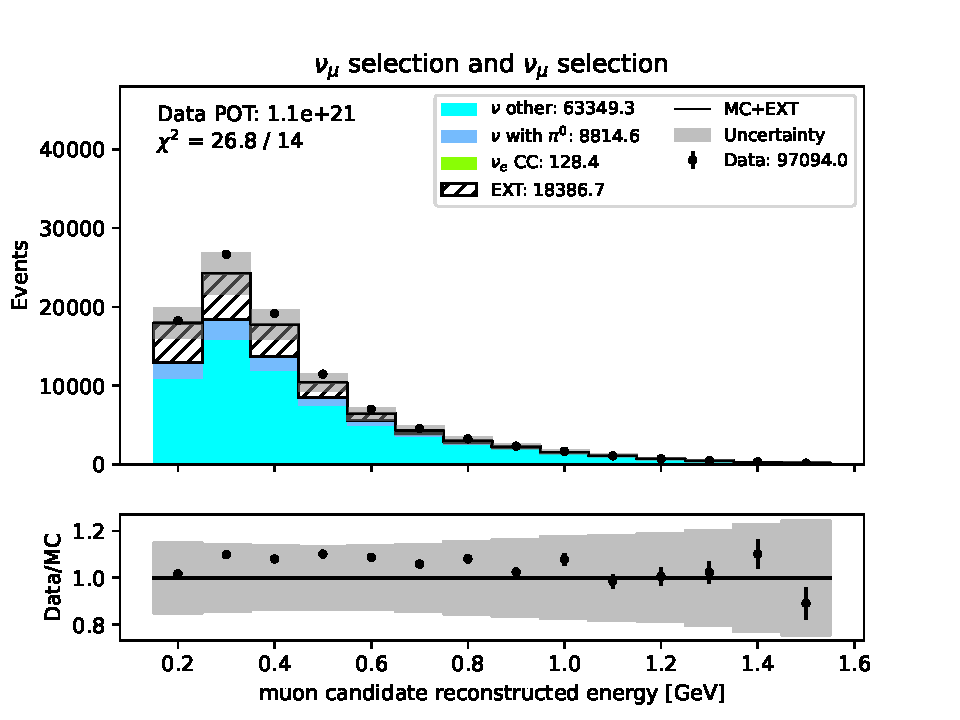
\includegraphics[width=\linewidth]{technote/Sidebands/Figures/NuMuSideband/muon_sideband_muon_energy_run1234b4c4d5_NUMU_NUMU.pdf}
        \caption{Muon reconstructed energy, runs 1-5.}
    \end{subfigure}%
    \begin{subfigure}{0.33\linewidth}
        \captionsetup{width=0.6\linewidth}
        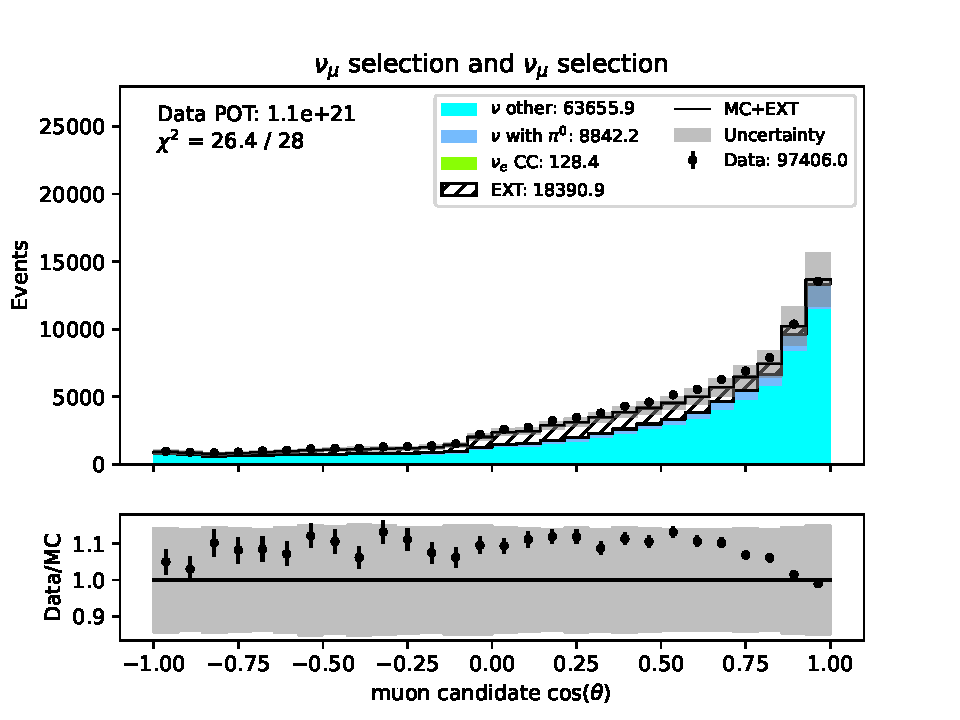
\includegraphics[width=\linewidth]{technote/Sidebands/Figures/NuMuSideband/muon_sideband_muon_theta_run1234b4c4d5_NUMU_NUMU.pdf}
        \caption{Muon candidate direction, runs 1-5.}
    \end{subfigure}%
    \begin{subfigure}{0.33\linewidth}
        \captionsetup{width=0.7\linewidth}
        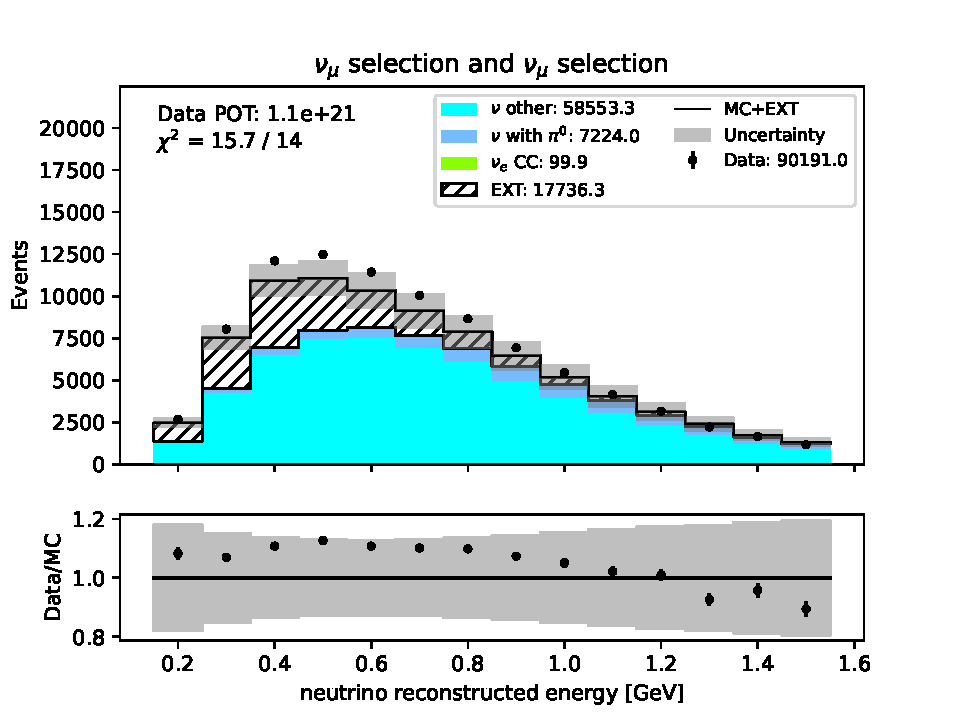
\includegraphics[width=\linewidth]{technote/Sidebands/Figures/NuMuSideband/muon_sideband_neutrino_energy_run1234b4c4d5_NUMU_NUMU.pdf}
        \caption{Reconstructed neutrino energy, runs 1-5.}
    \end{subfigure}
    \caption{Data and MC simulation comparisons after applying the muon sideband selection from Table~\ref{appendix:NuMuSelection}.}
    \label{fig:NuMuSideband}
\end{figure}